U ovom poglavlju biti će opisana istraživanja provedena u sklopu ovog rada. Za istraživanja je korišteno radno okruženje ECF (\textit{eng. Evolutionary Computation Framework}) koje je za potrebe ovog rada nadograđeno potrebnim, nedostajućim  operatorima križanja.

\section{ECF}
ECF \cite{ecf} (\textit{eng. Evolutionary Computation Framework}) predstavlja okruženje napisano u jeziku C++ za rješavanje različitih problema evolucijskog računanja. Za potrebe ovog rada, najznačajnije korišten dio ECF-a uključuje stablasti genotip (\textit{eng. tree}), zajedno s njegovim operatorima križanja i mutacije. Dio koji je nedostajao ovom okruženju za provedbu kasnije opisanih eksperimenata uključuje implementaciju homolognog, determinističkog, probabilističkog i semantičkog križanja. Iz tog razloga, kao praktičan dio ovog rada, ECF je nadograđen sa spomenutim operatorima križanja.

\section{Problemi za ispitivanje}

Kako bi se pokazala učinkovitost različitih operatora križanja nad različitim vrstama problema, ispitivanja su provedena nad različitim problemima simboličke regresije i logičke i programske domene. U nastavku je za svaku vrstu problema opisan specifičan problem koji je kasnije korišten za provedbu istraživanja. Nakon toga dana je detaljna analiza dobivenih rezultata, koja sadrži međusobnu usporedbu učinkovitosti različitih operatora križanja za svaki pojedini problem.

\subsection{Logičke funkcije}

\subsubsection{Multiplekser problem}
Kako bi se ispitala učinkovitost operatora križanja nad evolucijom logičkih funkcija, provedeni su eksperimenti nad 6 - multiplekser i 11 - multiplekser problemu \cite{koza}. Općenito, cilj $n$ - multiplekser problema je pronaći logičku funkciju koja za danih $n$ bitova (od kojih je određen broj adresnih i podatkovnih bitova) generira odgovarajući ulaz. Na slici \ref{muxPicture} prikazan je 6 - multiplekser, koji za 2 adresna bita na izlaz propušta jedan od 4 podatkovna bita.

\begin{figure}[H]
\centering
\begin{tikzpicture}
  % Inputs
  \draw[|-o] (-2,3.5) node[anchor=east] {$d_0$} -- (0.5,3.5);
  \draw[|-o] (-2,2.5) node[anchor=east] {$d_1$} -- (0.5,2.5);
  \draw[|-o] (-2,1.5) node[anchor=east] {$d_2$} -- (0.5,1.5);
  \draw[|-o] (-2,0.5) node[anchor=east] {$d_3$} -- (0.5,0.5);

  % Output
  \draw[o-|] (2.75,2) -- (5.25,2) node[anchor=west] {$y$};

  % Select
  \draw[|-o] (1,6) node[anchor=south] {$a_0$} -- (1,3.5);
  \draw[|-o] (2,6) node[anchor=south] {$a_1$} -- (2,3.5);

  % Rectangle
  \draw (0,0) rectangle node {Multiplekser} (3,4);
\end{tikzpicture}
\label{muxPicture}
\caption{6 - multiplekser}
\end{figure}

Primjerice, za adresne bitove $a_0=1$ i $a_1=0$, na izlaz bi se pustio drugi po redu podatkovni bit (01 binarno = 1 decimalno), odnosno $d_1$.

U tablici \ref{muxTable} prikazani su korišteni parametri za predstavljene 6 i 11 - multiplekser probleme.

\begin{table}[H]
 	\centering

    \begin{tabular}{| l | l | l |}
    \hline
   problem & 6 - multiplekser & 11 - multiplekser \\ \hline
   skup završnih znakova & $\{a_0, a_1, d_0, d_1, d_2, d_3 \}$ & $\{a_0, a_1, a_2, d_0, d_1, d_2, d_3, d_4, d_5, d_6, d_7 \}$\\ \hline
   skup nezavršnih znakova & $\{ AND, OR, NOT, IF \}$  & $\{ AND, OR, NOT, IF \}$ \\ \hline
   funkcija dobrote & broj netočnih izlaza & broj netočnih izlaza \\ \hline
    \end{tabular}
    
    \caption{Parametri $n$ multiplekser problema}
    \label{muxTable}
\end{table}

\subsubsection{Evolucija kriptografski sigurnih logičkih funkcija}
Za ispitivanje učinkovitosti operatora nad logičkim funkcijama također je korišten problem evolucije kriptografski sigurnih logičkih funkcija \cite{bool}. Cilj je pronaći neku logičku funkciju koja će imati dobra kriptografska svojstva. Svojstva koja posjeduje dobra kriptografska logička funkcija uključuju:

\begin{itemize}
\item{balansiranost - funkcija je balansirana ukoliko ima jednak broj istinitih i lažnih vrijednosti}
\item{visoku nelinearnost - linearnost logičke funkcije definira se kao postojanje $a_0,a_1,...,a_n \in \{0, 1\}$ tako da je $f(b_1,...,b_n) =  a_0 \oplus (a_1 \wedge b_1) \oplus ... \oplus (a_n \wedge b_n)$ za sve $b_1,....,b_n \in \{0, 1\}$}
\item{visok algebarski stupanj - algebarski stupanj logičke funkcije jednak je broju varijabli izraza s najvećim brojem varijabli u algebarskom normalnom obliku funkcije}
\item{visok algebarski imunitet - algebarski imunitet definiran je kao minimalni broj ne-nul funkcija $g$ takvih da su $fg = 0$ ili $(f\oplus 1)g=0$}
\item{visok korelacijski imunitet - korelacijski imunitet funkcije $f$ je maksimalna vrijednost $m$ takva da $| F\^(\omega) |= 0$ za sve vrijednosti Hammingove težine $\omega \leq m$ }
\end{itemize}

Budući da je nemoguće stvoriti logičku funkciju koja posjeduje sva ova svojstva, algoritmu se postavlja zadatak pronalaska dobre kombinacije nekih od ovih svojstava.

\subsection{Simbolička regresija}

\subsubsection{Klasična simbolička regresija}
Simbolička regresija je postupak pronalaženja matematičkog izraza iz danih empirijskih podataka. Za potrebe ovih mjerenja korištena je stablasta jedinka koja predstavlja jedan matematički izraz. Taj izraz se iz jedinke može jednostavno isčitati \textit{in-order} obilaskom stabla. Na slici \ref{symbTree} prikazana je jedinka koja predstavlja matematički izraz $cos(x-y) + (x / y)$.

\begin{figure}[H]
 	\centering

\begin{tikzpicture}
	[sibling distance=25mm, level distance=15mm,
	every node/.style={fill=blue!20,circle,draw,drop shadow, minimum height=1cm}]

	\node   {\textbf{+}}
    		child {node {$cos$}
    			child {node {-}
    				child {node {x}}
    				child {node {y}}
    			}
    		}
    		child {node {\textbf{$/$}}
			child {node  {x}}
			child {node  {y}}	
		};
	};

\end{tikzpicture}


	\caption{Primjer jedinke koja rješava problem simboličke regresije koja predstavlja izraz $cos(x-y) + (x / y)$}
	\label{symbTree}
\end{figure}

U tablici \ref{bla} \footnote{mse označava kvadratičnu sumu odstupanja (\textit{eng. mean square error})} su dani izrazi koji su bili ciljna funkcija u provedenim istraživanjima, zajedno s njihovim intervalom domene i oznakama koje su kasnije korištene za jednostavnije referenciranje.

\begin{table}[H]
 	\centering

    \begin{tabular}{| l | l | l | l |}
    \hline
    oznaka & izraz & interval domene & funkcija dobrote\\ \hline
    symb1 & $log(x+1)+log(x^2+1)$ & $x \in [0, 20]$ & $mse$ \\ \hline
    symb2 & $sin(x) + sin(y^2)$ & $x, y \in [-10, 10]$ & $mse$\\ \hline
    symb3 & $2 \cdot sin(x) \cdot cos(y)$ & $x, y \in [-10, 10]$ & $mse$\\ \hline
    symb4 & $x \cdot y + sin((x+1) \cdot (y-1))$ & $x, y \in [-10, 10]$ & $mse$\\ \hline
    symb5 & \Large{ $\frac{8}{2 + x^2 + y^2}$ }& $x, y \in [-10, 10]$ & $mse$\\ \hline
    symb6 & $\frac{x^3}{5} + \frac{y^3}{2} - x - y$ & $x, y \in [-10, 10]$ & $mse$\\ \hline
    \end{tabular}
    
    \caption{Popis problema simboličke regresije}
    \label{bla}
\end{table}

\subsubsection{Evolucija funkcije prioriteta za uporabu unutar pravila raspoređivanja}
Cilj ovog problema jest pronaći funkciju prioriteta koja će se upotrijebiti unutar pravila raspoređivanja \cite{jakobovic}. Pritom, pravila već imaju predefiniranu globalnu strukturu, dok se pojedini dijelovi evoluiraju genetskim programiranjem. Postupak raspoređivanja kojega algoritmi koriste je prioritetno raspoređivanje (\textit{engl. priority scheduling}), pri kojemu se zadano trenutno stanje sustava preslikava u sljedeće stanje. Prijelaz iz jednoga u drugo stanje definiran je pridruživanjem određene aktivnosti nekome sredstvu, a odabir aktivnosti i sredstva obavlja se računanjem prioriteta svakog raspoloživog sredstva i aktivnosti, ovisno o dotičnom okruženju. Ovisno o kriteriju raspoređivanja, funkcija prioriteta se pronalazi automatski, uz pomoć genetskog programiranja.


\subsection{Programi}
Programski problem korišten za evaluaciju operatora križanja bio je problem umjetnog mrava (\textit{eng. Artificial Ant Problem}). Rješenje ovog problema jest evoluirati program koji opisuje ponašanje mrava u nekoj okolini koja sadrži hranu. Dobar program bi trebao biti sposoban pronaći i pojesti što više hrane iz okoline. Jedinka je u ovom slučaju također predstavljena kao stablo. Primjer jedinke prikazan je na slici \ref{ant}. Dobrota jedne ovakve jedinke jednaka je broju pojedene hrane u testnoj, prilikom učenja ne viđenoj okolini.

\begin{figure}[H]
	\centering

\begin{tikzpicture}
[sibling distance=50mm, level distance=25mm,
every node/.style={fill=blue!20,rectangle, rounded corners,draw,drop shadow, minimum height=1.5cm}]


  \node {ifFoodAhead}
      child {node {moveForward}}
      child {node {Prog2}
        child {node {turnRight}}
        child {node {ifFoodAhead}
        	child{node {moveForward}}
        	child{node {turnLeft}}
        }
      };
\end{tikzpicture}

	\caption{Primjer jedinke programa umjetnog mrava}
	\label{ant}
\end{figure}

Nezavršni znakovi koji grade jednu ovakvu jedinku su:

\begin{enumerate}

  \item \textbf{If food ahead} - provjerava da li se nalazi hrana ispred mrava - ako da izvršava lijevu granu, ako ne, izvršava desnu granu.
  \item \textbf{Prog2} - slijedno izvršava lijevu, te zatim desnu granu.
  \item \textbf{Prog3} - slijedno izvršava (s lijeva na desno) svaku od 3 pridružene grane.

\end{enumerate}

Završni znakovi koji grade ovu jedinku su:
\begin{enumerate}

  \item \textbf{move forward} - pomiče mrava za jedno mjesto unaprijed.
  \item \textbf{turn right} - okreće mrava u desno.
  \item \textbf{turn left} - okreće mrava u lijevo.

\end{enumerate}

%Pseudokod koji predstavlja ponašane jedinke prikazane na slici \ref{ant} prikazan je na \ref{pseudokod}.

%\begin{algorith m}
%\eIf {food ahead} {
%	move forward;
%} {
%	turn right;\\
%	\eIf {food ahead} {
%		move forward;
%	} {
%		turn left;
%	}
%}

%	\caption{Pseudokod jedinke prikazane na slici \ref{ant}}
%	\label{pseudokod}
%	\centering
%\end{algorithm}


\section{Rezultati}
\subsection{Usporedba učinkovitosti pojedinačnih operatora križanja}
U ovom poglavlju dan je pregled provedenih eksperimenata u sklopu ovog rada. Za svaki problem dani su parametri izvođenja pojedinog eksperimenta, te su grafički i opisno prikazani njegovi rezultati.

Valja napomenuti kako se semantičko križanje koristilo u kombinaciji s jednostavnim križanjem s omjerom vjerojatnosti semantičko križanje : jednostavno križanje = 1 : 9. Razlog ovome je to što se nakon izvršavanja semantičkog križanja nije provodilo pojednostavljivanje stabala što je dovodilo do eksponencijalnog rasta stabala jedinki.
\subsubsection{Logičke funkcije}
\textbf{6 - multipleksor}

Na slici \ref{muxbox} prikazani su rezultati usporedbe operatora nad problemom 6 - multipleksor. Za ovaj eksperiment korišteni su konstanti parametri:
\begin{itemize}
\item{veličina populacije = 400}
\item{broj generacija = 15}
\item{faktor mutacije = 0.4}
\end{itemize}


Razlog uporabe ovako malog broja generacije jest činjenica da je ovaj problem donekle jednostavan, te za veći broj generacija u većini slučajeva svaki operator uspije pronaći točno rješenje ovog problema. Kako bi usporedba učinkovitosti operatora bila moguća, evolucija je prekinuta na petnaestoj generaciji.

Iz rezultata je uočljivo kako je kombinacija semantičkog i jednostavnog križanja u omjeru 1:9 daleko sporije konvergirala točnom rješenju nego ostali operatori. Razlog ovome je vjerojatno činjenica što ovaj operator spaja dvije roditeljske jedinke u novu, čime se u biti ne modificira ponašanje dobre jedinke, već udvostručava donekle dobro ponašanje dvije dobre jedinke.

\begin{figure}[H]
	\centering
	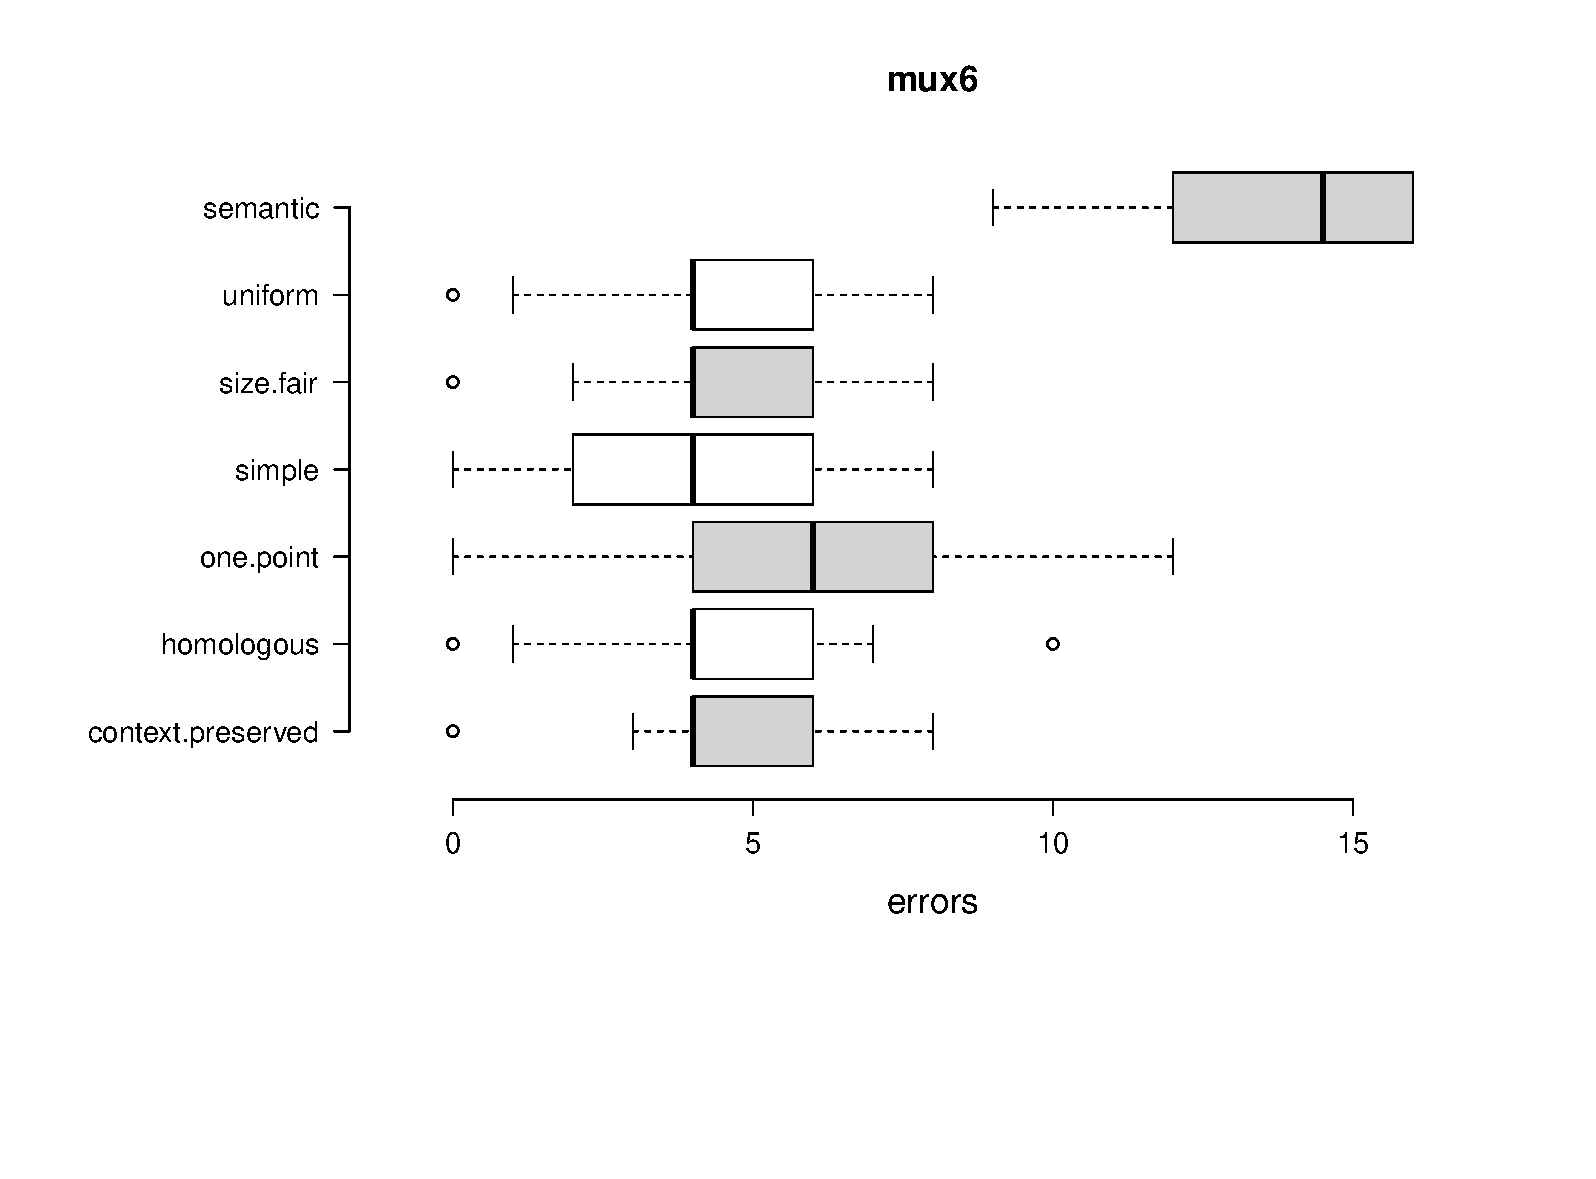
\includegraphics[trim=0cm 4cm 0cm 0cm, scale=0.6]{./slike/boxPlots/mux6.eps}
	\caption{Usporedba učinkovitosti pojedinačnih operatora križanja na problem 6 - multipleksora}
	\label{muxbox}
\end{figure}

\textbf{11 - multipleksor}


\textbf{Evolucija kriptografski sigurnih logičkih funkcija - inačica 1}



\textbf{Evolucija kriptografski sigurnih logičkih funkcija - inačica 4}

\subsubsection{Simbolička regresija}

\textbf{Klasična simbolička regresija}


Na grafovima u nastavku prikazana je učinkovitost pojedinih operatora križanja na probleme klasične simboličke regresije predstavljene na početku poglavlja. Svaki eksperiment pokrenut je 30 puta. U ovom slučaju, potrebno je minimizirati funkciju dobrote koja se računa kao srednja kvadratna pogreška. U svim slučajevima, probabilističko križanje pokazalo se kao daleko najlošije - dobrota jedinki dobivenih ovim križanjem redovito je odskakala od ostalih za jedan red veličine. Radi toga, na grafovima u nastavku nije uključeno to križanje iz razloga što bi pokvarilo njihovu razlučivost.

Na slici \ref{symb1box} prikazana je učinkovitost operatora križanja prilikom rješavanja prvog problema simboličke regresije (symb1). Za ovaj eksperiment korišteni su konstanti parametri:
\begin{itemize}
\item{veličina populacije = 400}
\item{broj generacija = 200}
\item{faktor mutacije = 0.5}
\end{itemize}

Vidljivo je kako je za ovaj problem daleko najučinkovitiji bio operator semantičkog križanja, odnosno kombinacije semantičkog i jednostavnog križanja u omjeru 1:9. 

\begin{figure}[H]
	\centering
	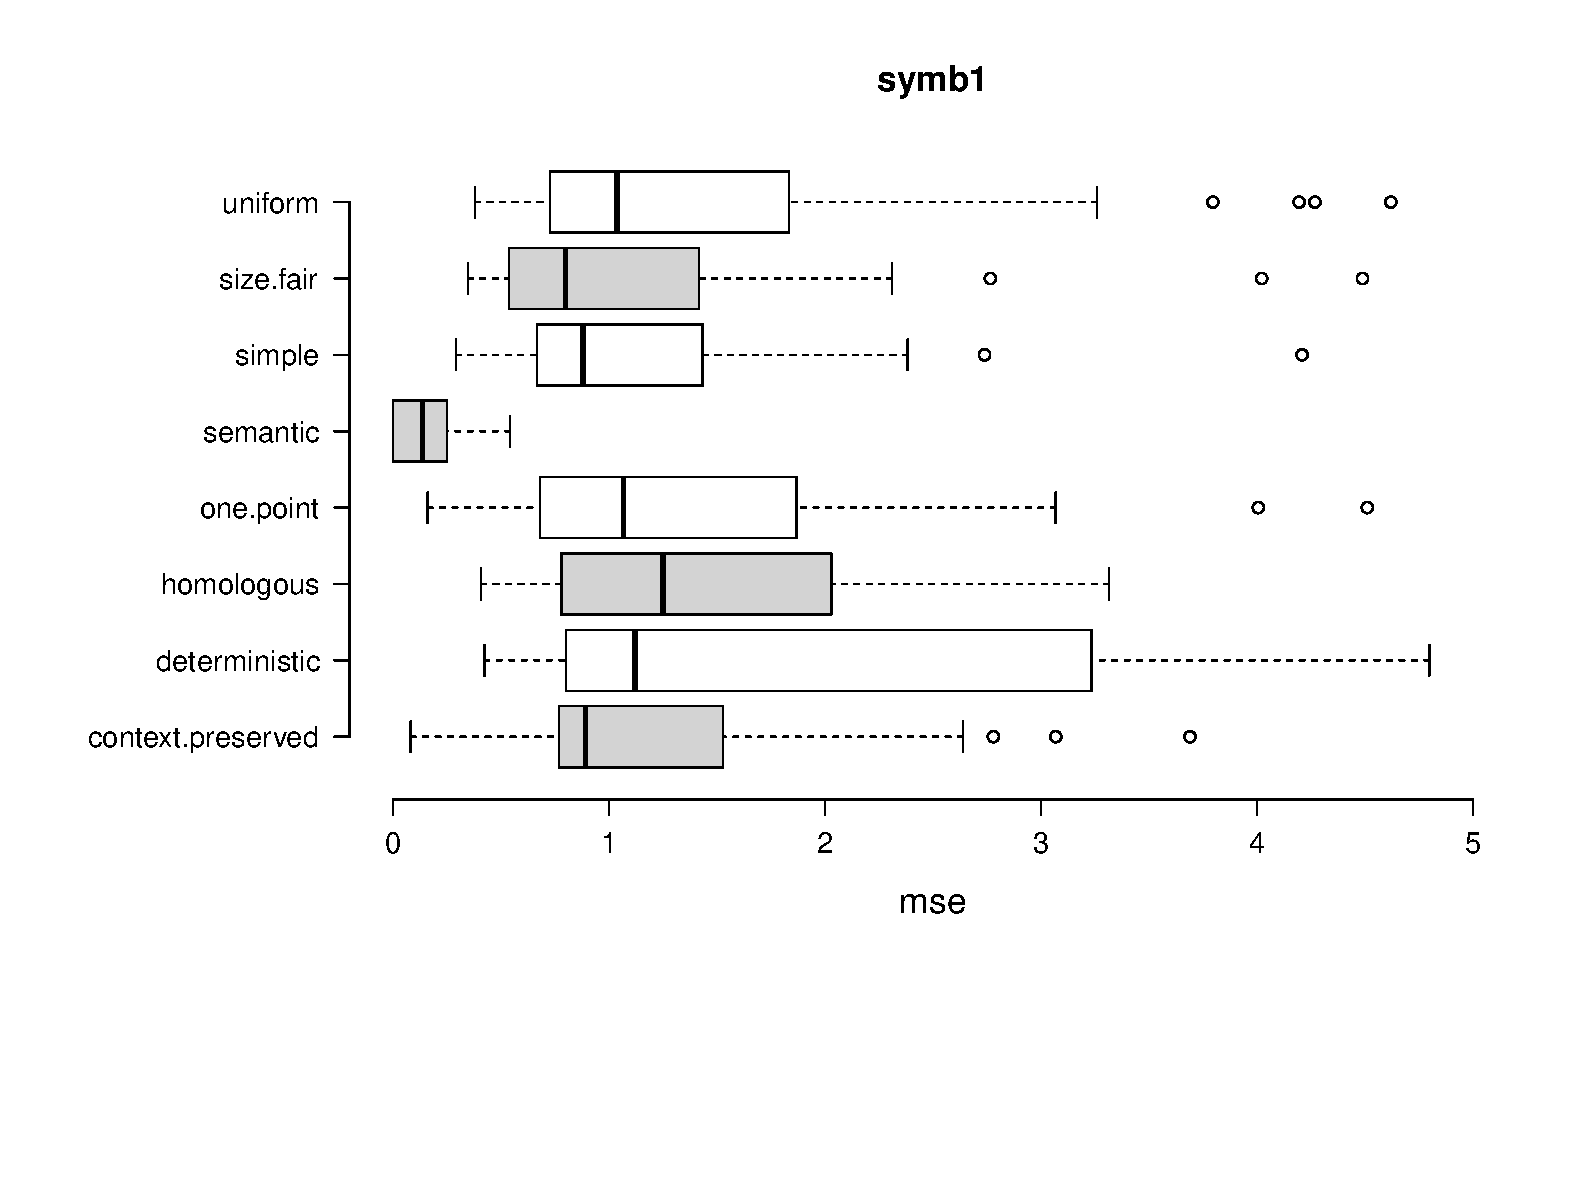
\includegraphics[trim=0cm 4cm 0cm 0cm, scale=0.6]{./slike/boxPlots/symb1.eps}
	\caption{Usporedba učinkovitosti pojedinačnih operatora križanja na problem simboličke regresije symb1}
	\label{symb1box}
\end{figure}


\begin{figure}[H]
	\centering
	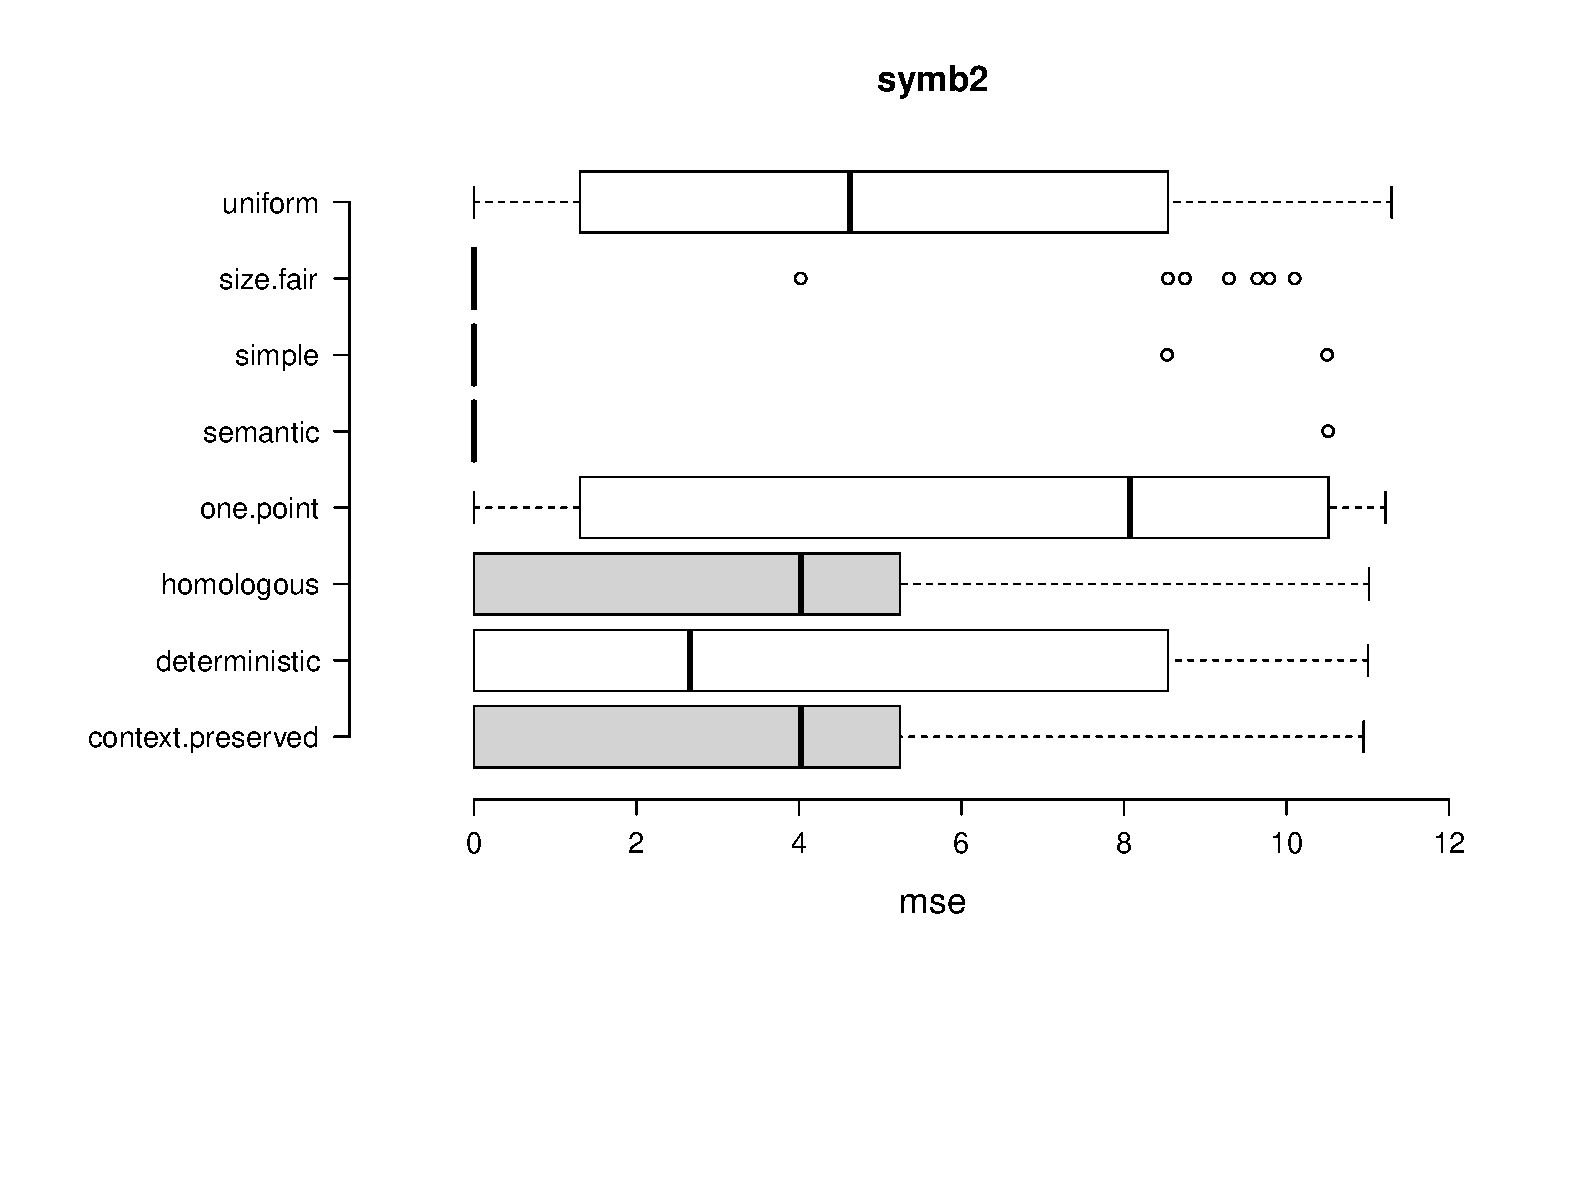
\includegraphics[trim=0cm 4cm 0cm 0cm, scale=0.6]{./slike/boxPlots/symb2.eps}
	\caption{Usporedba učinkovitosti pojedinačnih operatora križanja na problem simboličke regresije symb2}
	\label{symb2box}
\end{figure}


Na slici \ref{symb2box} prikazana je usporedba učinkovitosti operatora na problemu simboličke regresije symb2. Za ovaj eksperiment korišteni su konstanti parametri:
\begin{itemize}
\item{veličina populacije = 100}
\item{broj generacija = 50}
\item{faktor mutacije = 0.2}
\end{itemize} 

Na slici \ref{symb2box} jednostavno križanje, križanje pravedno s obzirom na veličinu i kombinacija semantičkog i jednostavnog križanja postigli su najbolje rezultate. Ostali operatori su se pokazali kao znatno lošiji prilikom rješavanja ovog problema.


\begin{figure}[H]
	\centering
	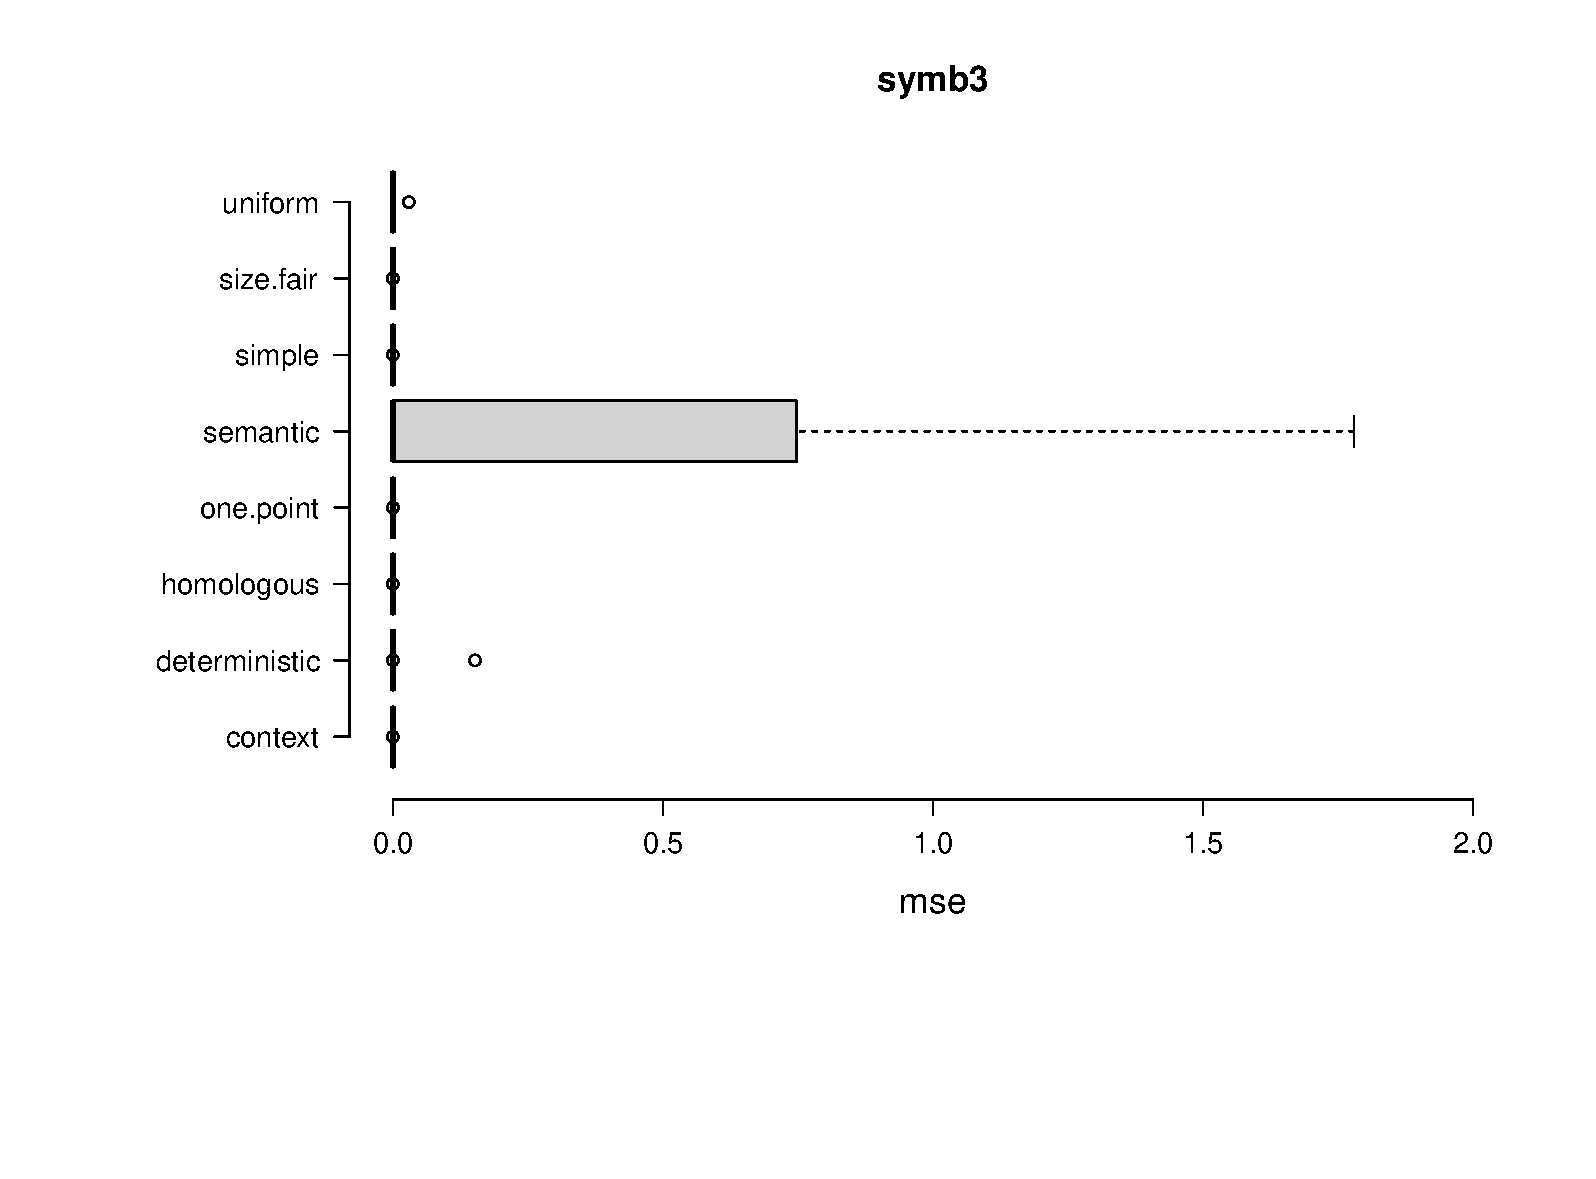
\includegraphics[trim=0cm 4cm 0cm 0cm, scale=0.6]{./slike/boxPlots/symb3.eps}
	\caption{Usporedba učinkovitosti pojedinačnih operatora križanja na problem simboličke regresije symb3}
	\label{symb3box}
\end{figure}

Na slici \ref{symb3box} prikazana je usporedba učinkovitosti operatora na problemu simboličke regresije symb3. Za ovaj eksperiment korišteni su konstanti parametri:
\begin{itemize}
\item{veličina populacije = 400}
\item{broj generacija = 50}
\item{faktor mutacije = 0.3}
\end{itemize} 

Vidljivo je kako je ovaj problem ispao prilično lagan za sve operatore - jedini operator koji je bio nešto neučinkovitiji bio je semantički operator križanja (odnosno, njegova kombinacija s jednostavnim križanjem u omjeru 1:9) koji u nekoliko pokretanja nije uspio pronaći točno rješenje.


\begin{figure}[H]
	\centering
	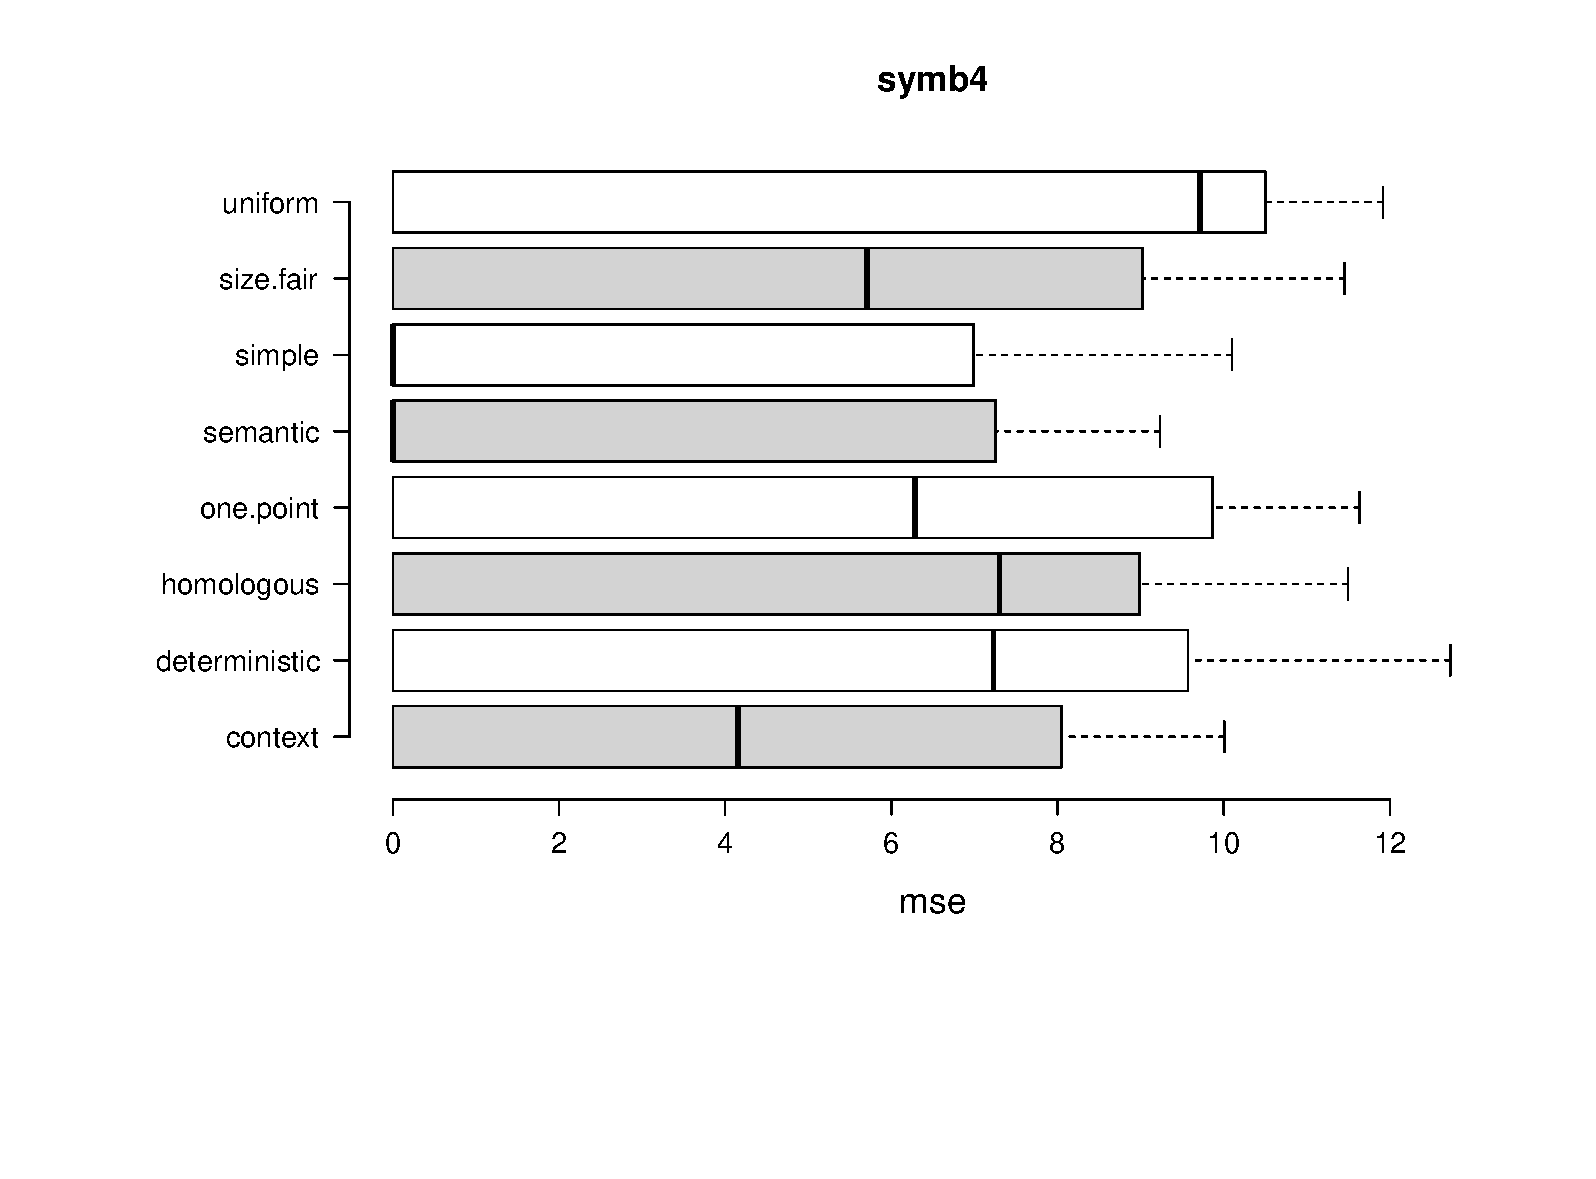
\includegraphics[trim=0cm 4cm 0cm 0cm, scale=0.6]{./slike/boxPlots/symb4.eps}
	\caption{Usporedba učinkovitosti pojedinačnih operatora križanja na problem simboličke regresije symb4}
	\label{symb4box}
\end{figure}

Na slici \ref{symb4box} prikazana je usporedba učinkovitosti operatora na problemu simboličke regresije symb4. Za ovaj eksperiment korišteni su konstanti parametri:
\begin{itemize}
\item{veličina populacije = 500}
\item{broj generacija = 200}
\item{faktor mutacije = 0.2}
\end{itemize} 

Vidiljivo je kako su statistički najbolji operatori jednostavno križanje i kombinacija semantičkog i jednostavnog križanja u omjeru 1:9. 


\begin{figure}[H]
	\centering
	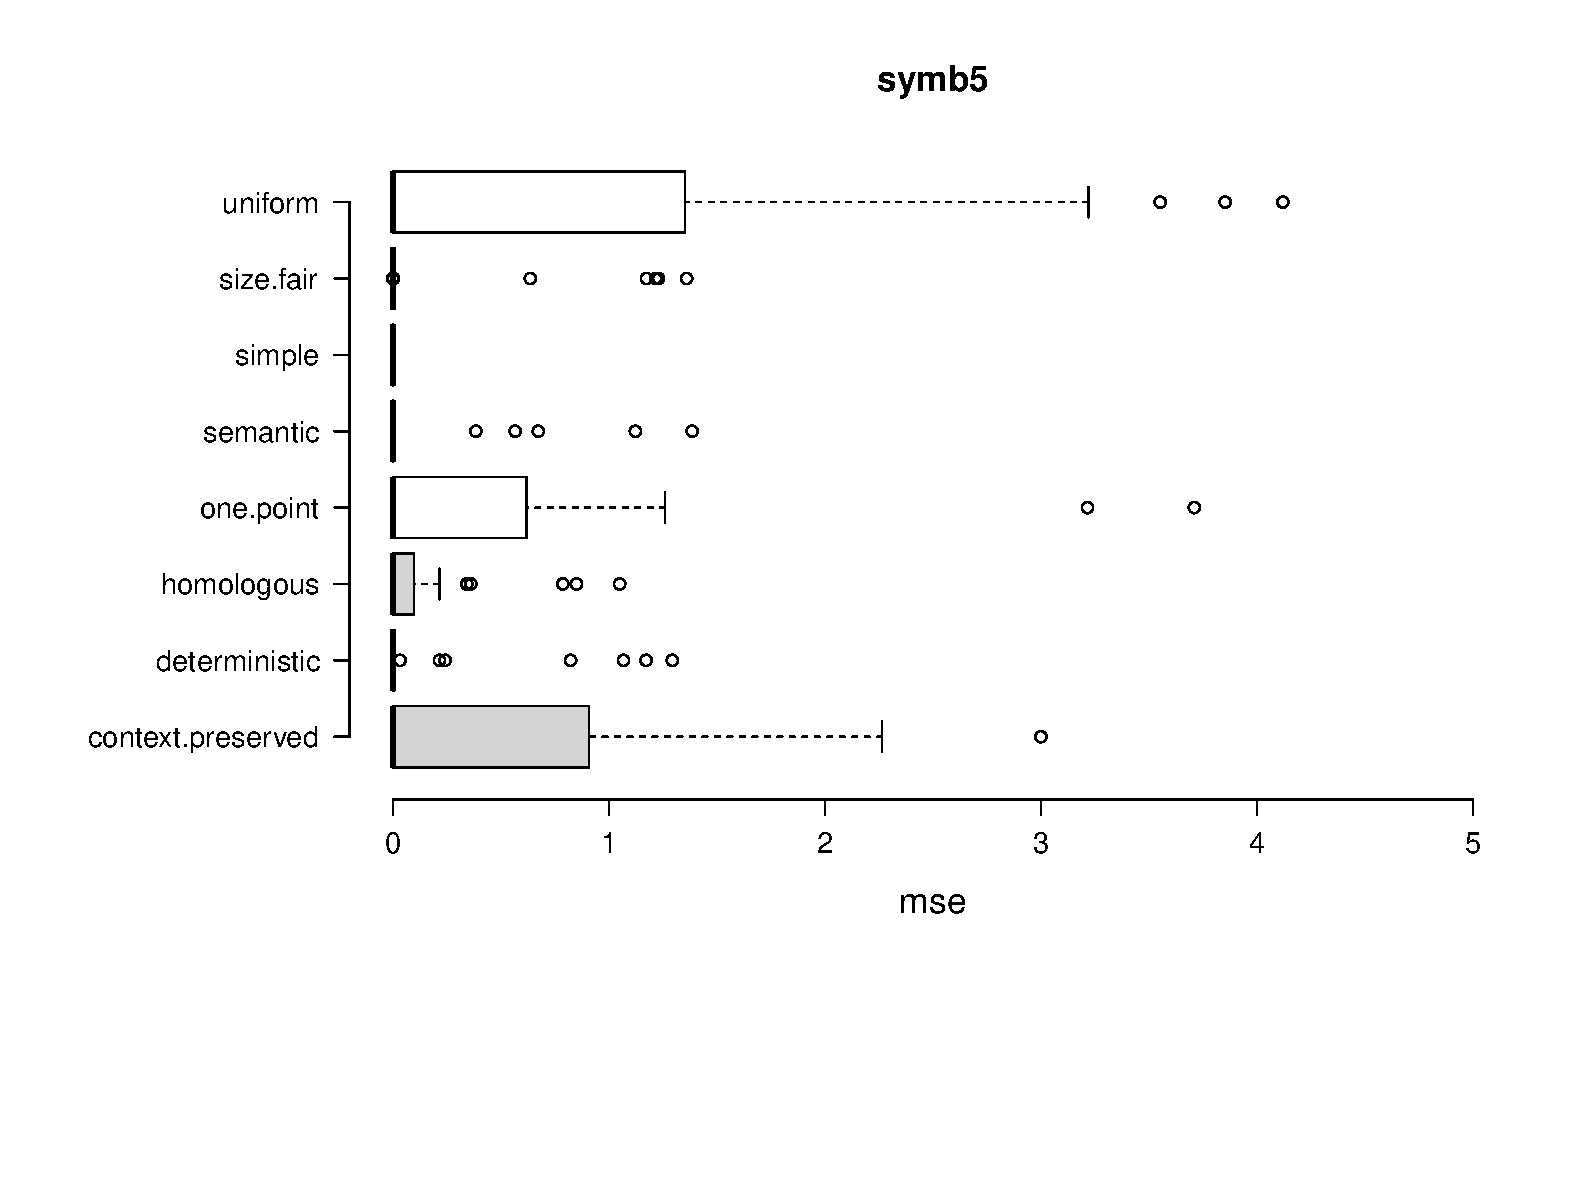
\includegraphics[trim=0cm 4cm 0cm 0cm, scale=0.6]{./slike/boxPlots/symb5.eps}
	\caption{Usporedba učinkovitosti pojedinačnih operatora križanja na problem simboličke regresije symb5}
	\label{symb5box}
\end{figure}


Na slici \ref{symb5box} prikazana je usporedba učinkovitosti operatora na problemu simboličke regresije symb5. Za ovaj eksperiment korišteni su konstanti parametri:
\begin{itemize}
\item{veličina populacije = 500}
\item{broj generacija = 200}
\item{faktor mutacije = 0.4}
\end{itemize} 

U prosjeku, rješenje ovog problema uspješno su pronašli svi operatori. Operatori uniformnog križanja, križanja s jednom točkom prekida i križanja s očuvanjem konteksta pritom su u nekim slučajevima dali nešto lošija rješenja.


\begin{figure}[H]
	\centering
	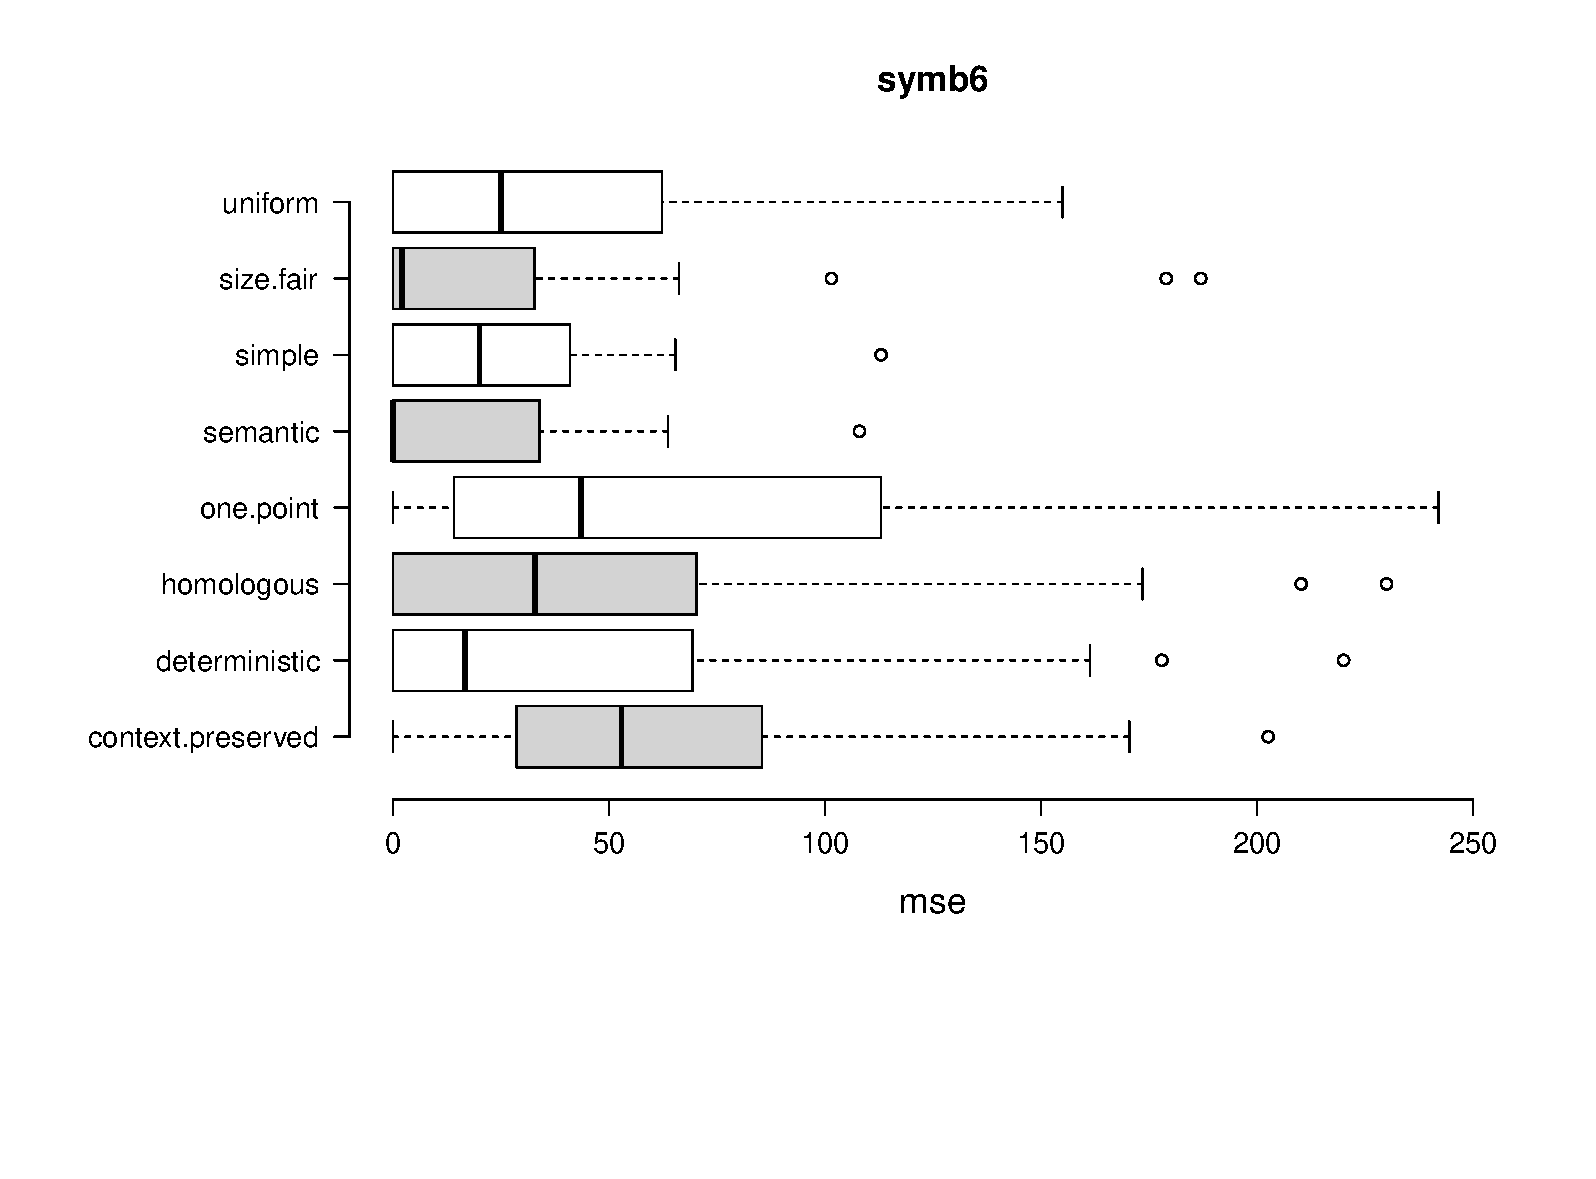
\includegraphics[trim=0cm 4cm 0cm 0cm, scale=0.6]{./slike/boxPlots/symb6.eps}
	\caption{Usporedba učinkovitosti pojedinačnih operatora križanja na problem simboličke regresije symb6}
	\label{symb6box}
\end{figure}


Na slici \ref{symb6box} prikazana je usporedba učinkovitosti operatora na problemu simboličke regresije symb6. Za ovaj eksperiment korišteni su konstanti parametri:
\begin{itemize}
\item{veličina populacije = 300}
\item{broj generacija = 200}
\item{faktor mutacije = 0.4}
\end{itemize} 

Za ovaj problem, najbolje se pokazalo semantičko križanje u kombinaciji s jednostavnim križanjem, koje je u prosjeku uvijek našlo točno rješenje.


U svim prethodno prikazanim rezultatima, najčešće se kao najučinkovitiji operator pokazao jednostavni operator križanja. Za njim slijedi kombinacija semantičkog križanja s jednostavnim križanjem, koje je u nekim slučajevima znala pronaći i bolje rješenje nego čisto jednostavno križanje. Iako bi se moglo zaključiti kako je ova kombinacija operatora učinkovita iz razloga što će u većini slučajeva upotrijebiti jednostavno križanje (koje se pokazalo kao najbolje križanje za rješavanje problema simboličke regresije) u nekim slučajevima (konkretno, symb2 i symb6) bilo je bolje od čistog jednostavnog križanja. To dokazuje kako je semantička komponenta te kombinacije nezanemariva i korisna.



\textbf{Evolucija funkcije prioriteta za uporabu unutar pravila raspoređivanja}



\subsubsection{Programi}
\textbf{Problem umjetnog mrava}

Na slici \ref{antbox} prikazana je usporedba učinkovitosti operatora križanja na rješavanje problema umjetnoga mrava. Prikazane vrijednosti su vrijednosti na skupu za učenje, a konstantni parametri korišteni za ovaj eksperiment su:
\begin{itemize}
\item{veličina populacije = 400}
\item{broj generacija = 100}
\item{faktor mutacije = 0.4}
\end{itemize} 

Budući da je cilj algoritma maksimizirati funkciju dobrote (koja se računa kao količina pojedene hrane unutar okoline za učenje), na grafu \ref{antbox} vidljivo je kako je najučinkovitiji operator za tu zadaću jednostavno križanje. Odmah nakon njega dolazi kombinacija semantičkog i jednostavnog križanja u omjeru 1:9 te križanje pravedno s obzirom na veličinu. Križanje s jednom točkom prekida pokazalo se kao najgore u ovom slučaju.

\begin{figure}[H]
	\centering
	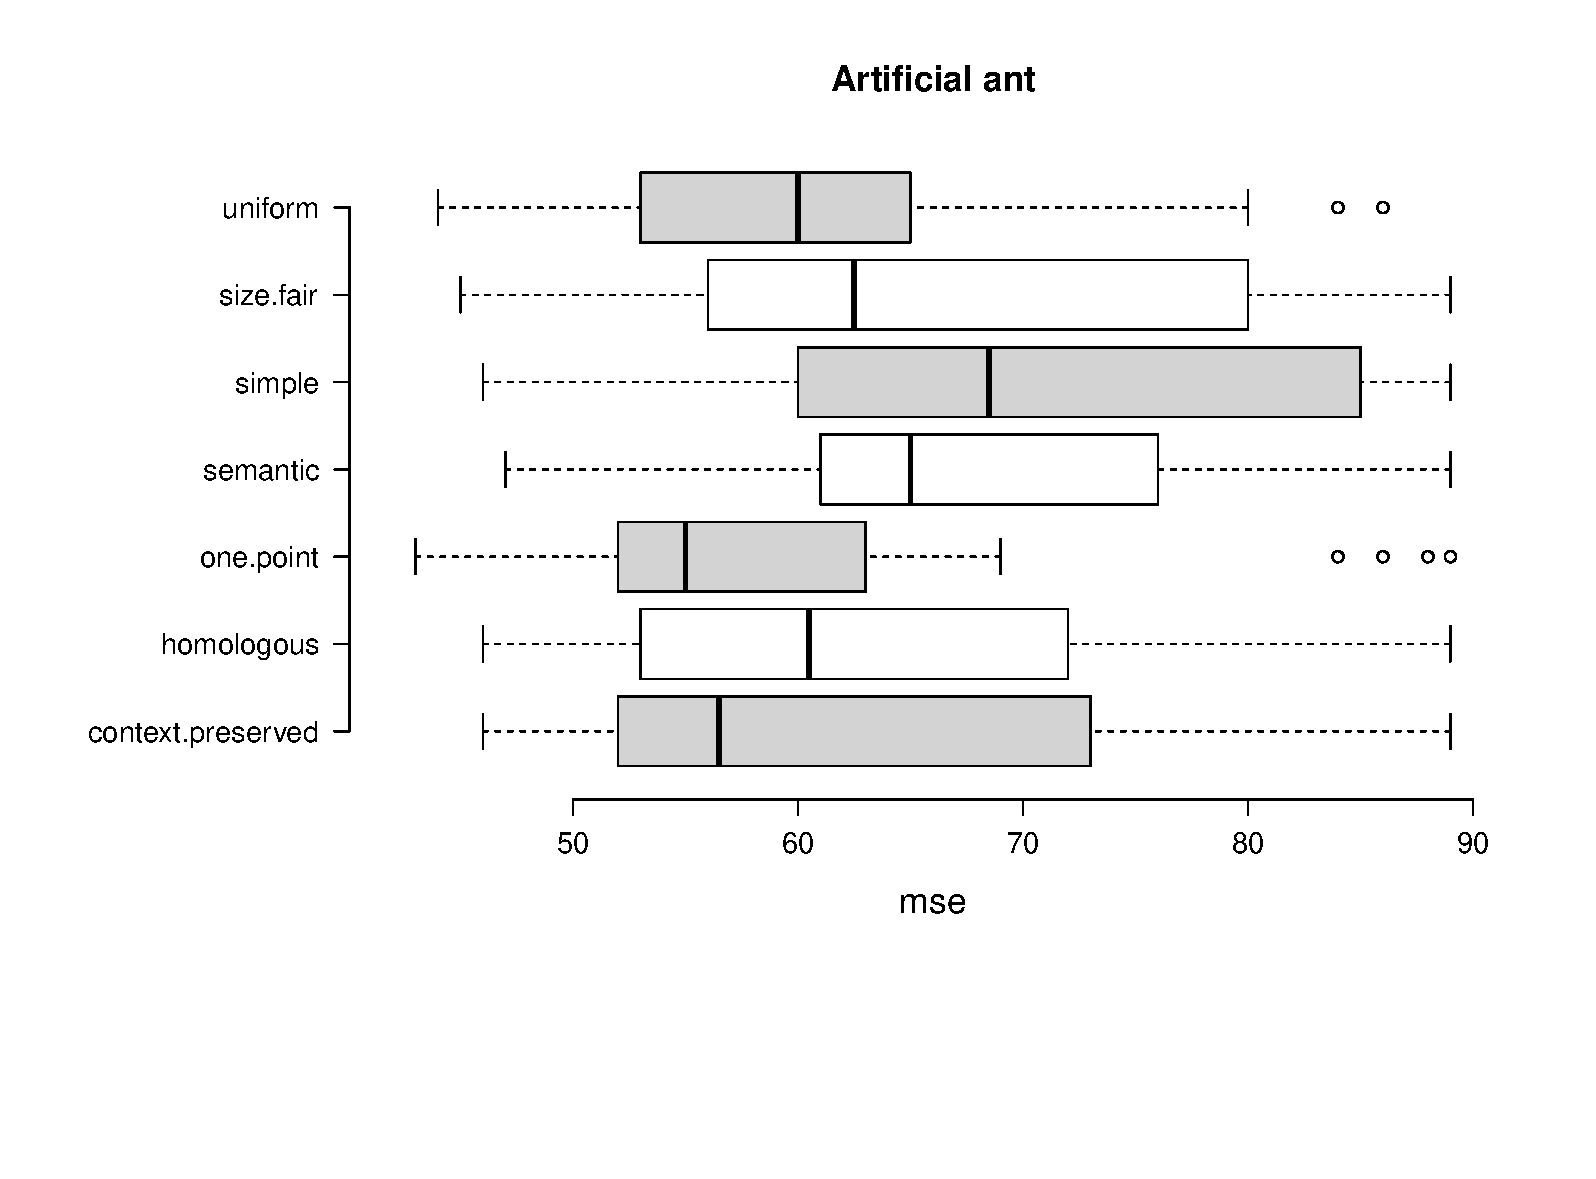
\includegraphics[trim=0cm 4cm 0cm 0cm, scale=0.6]{./slike/boxPlots/ant.eps}
	\caption{Usporedba učinkovitosti pojedinačnih operatora križanja na problem umjetnog mrava}
	\label{antbox}
\end{figure}

Osim ovog eksperimenta, proveden je eksperiment za usporedbu učinkovitosti trenutno najbolje evoluirane jedinke na okolini za učenje, te na dvije, još neviđene okoline za testiranje kroz 100 generacija za svaki operator križanja. Konstanti parametri za ovaj eksperiment jednaki su kao i u prethodnom slučaju. Na slici \ref{trails} prikazana je okolina za učenje i dvije testne okoline.

\begin{figure}[H]
	\centering
	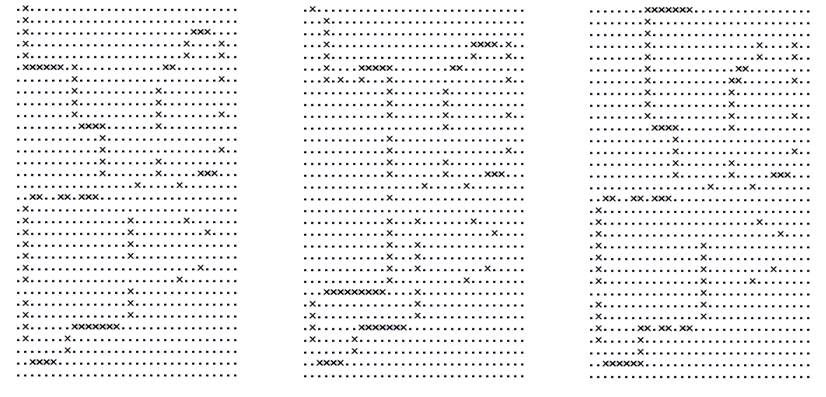
\includegraphics[scale=0.5]{./slike/cross-validation/trails.png}
	\caption{Lijevo: okolina za učenje, sredina: prva testna okolina, desno: druga testna okolina}
	\label{trails}
\end{figure}

Na sljedećim slikama prikazani su rezultati ovih eksperimenata. Na svakoj slici, plavom bojom prikazan je broj pojedene hrane na okolini za učenje, crvenom bojom broj hrane pojedene na prvoj testnoj okolini i zelenom bojom na drugoj testnoj okolini. Ovaj eksperiment proveden je iz razloga što evolucijom jedinke unutar okoline za učenje može doći do njenog prenaučavanja na tu okolinu. Iz tog razloga, kako bi se dobila realnija slika o učinkovitosti operatora, potrebno je usporediti učinkovitost evoluirane jedinke i na nekoj drugoj, jedinci još neviđenoj okolini.

Prikazani rezultati pokazuju kako nijedan operator nije značajno prenaučio najbolju evoluiranu jedinku. Kao što je i očekivano, u okolini za učenje učinkovitost najbolje jedinke u svakom je slučaju nešto veća nego ona u testnim okolinama. To upućuje na laganu prilagodbu jedinke na danu učeču okolinu.
\begin{figure}[H]
	\centering
	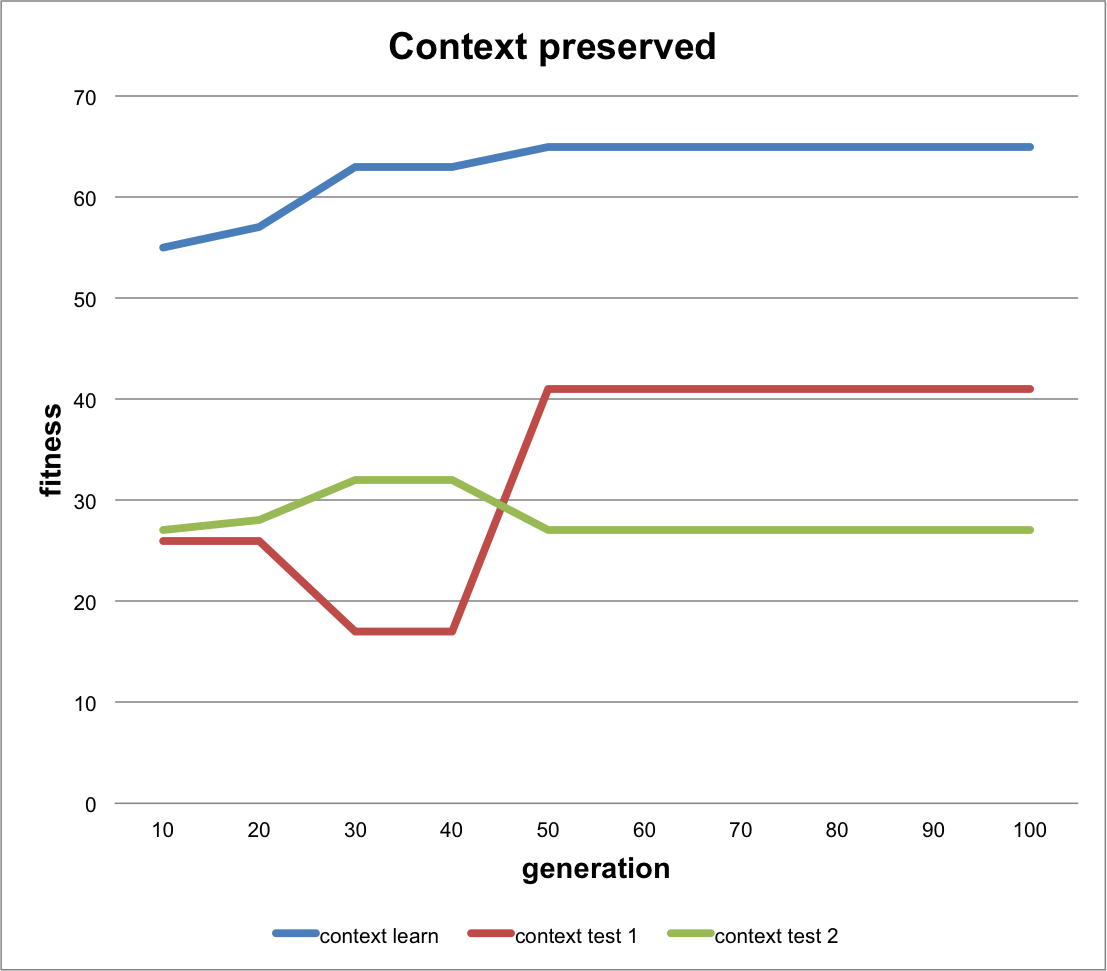
\includegraphics[scale=0.8]{./slike/cross-validation/context.png}
	\caption{Usporedba kvalitete evoluirane jedinke na okolini za učenje i dvije testne okoline za operator križanja s očuvanjem konteksta}
	\label{context}
\end{figure}

\begin{figure}[H]
	\centering
	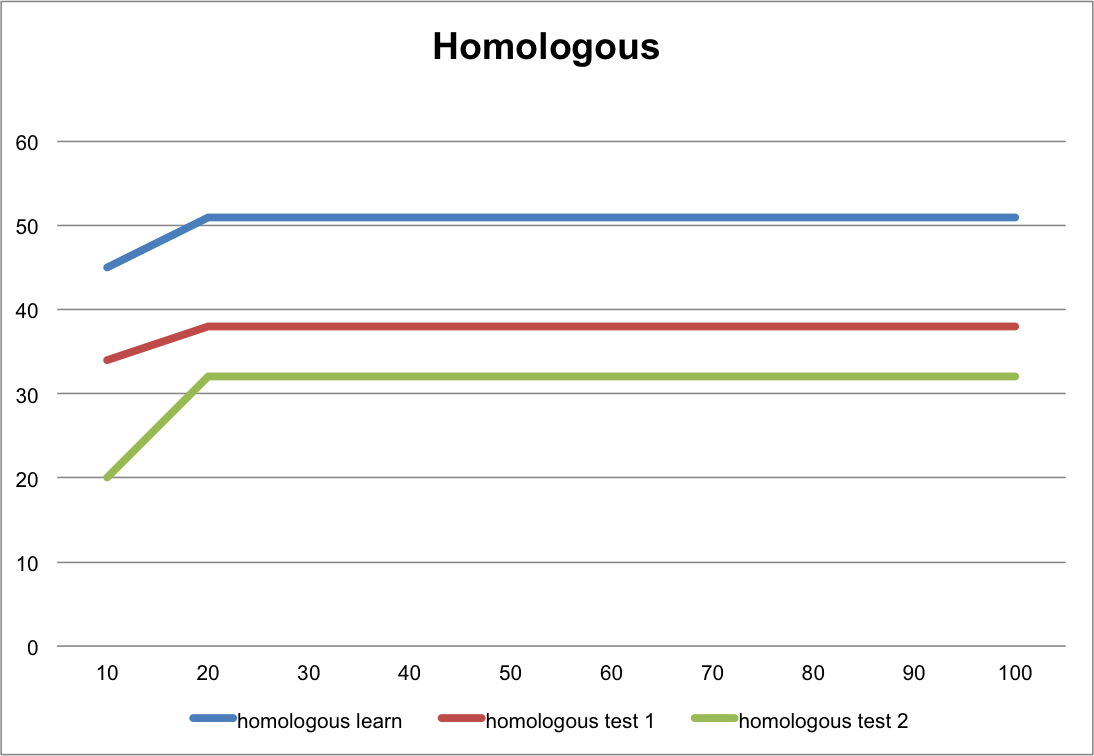
\includegraphics[scale=0.8]{./slike/cross-validation/homo.png}
	\caption{Usporedba kvalitete evoluirane jedinke na okolini za učenje i dvije testne okoline za homologni operator križanja}
	\label{homo}
\end{figure}

\begin{figure}[H]
	\centering
	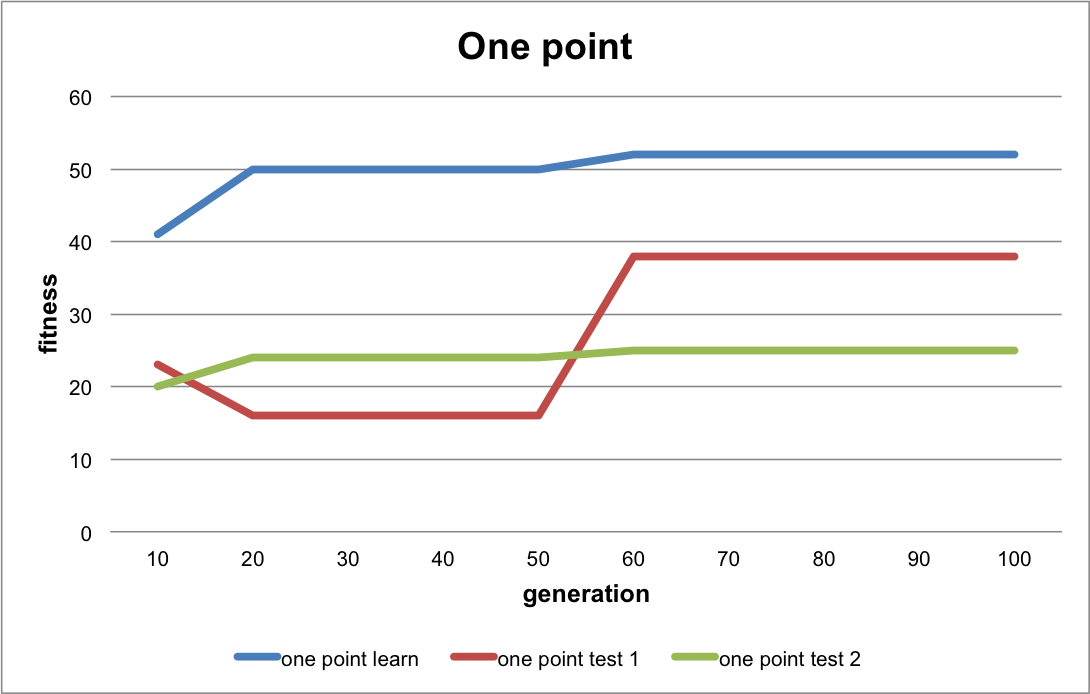
\includegraphics[scale=0.8]{./slike/cross-validation/onepoint.png}
	\caption{Usporedba kvalitete evoluirane jedinke na okolini za učenje i dvije testne okoline za operator križanja s jednom točkom prekida}
	\label{onepoint}
\end{figure}

\begin{figure}[H]
	\centering
	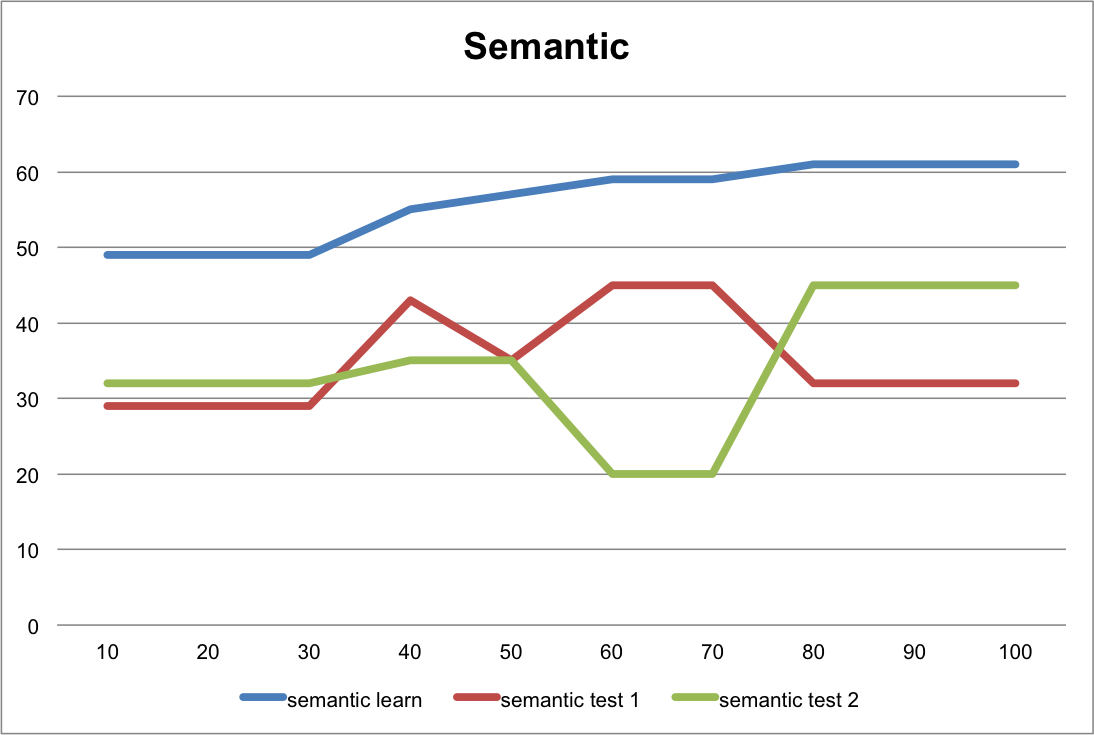
\includegraphics[scale=0.8]{./slike/cross-validation/semantic.png}
	\caption{Usporedba kvalitete evoluirane jedinke na okolini za učenje i dvije testne okoline za kombinaciju semantičkog i jednostavnog križanja u omjeru 1:9}
	\label{semantic}
\end{figure}

\begin{figure}[H]
	\centering
	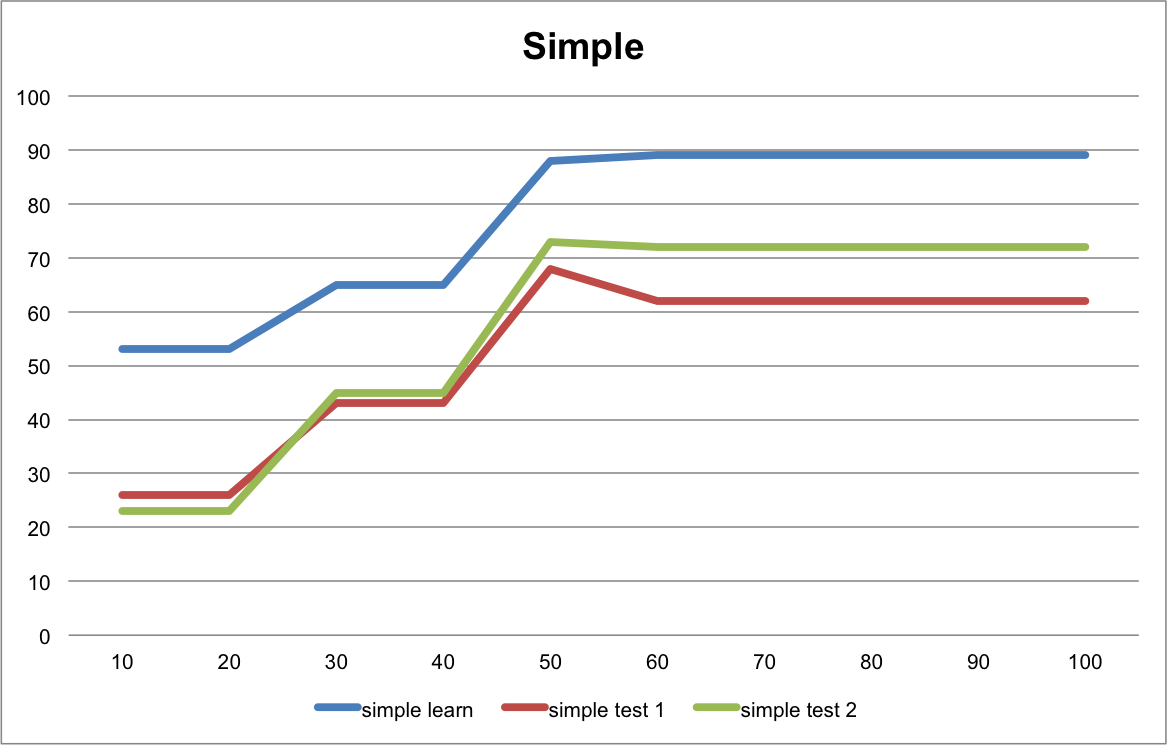
\includegraphics[scale=0.8]{./slike/cross-validation/simple.png}
	\caption{Usporedba kvalitete evoluirane jedinke na okolini za učenje i dvije testne okoline za jednostavni operator križanja}
	\label{simple}
\end{figure}

\begin{figure}[H]
	\centering
	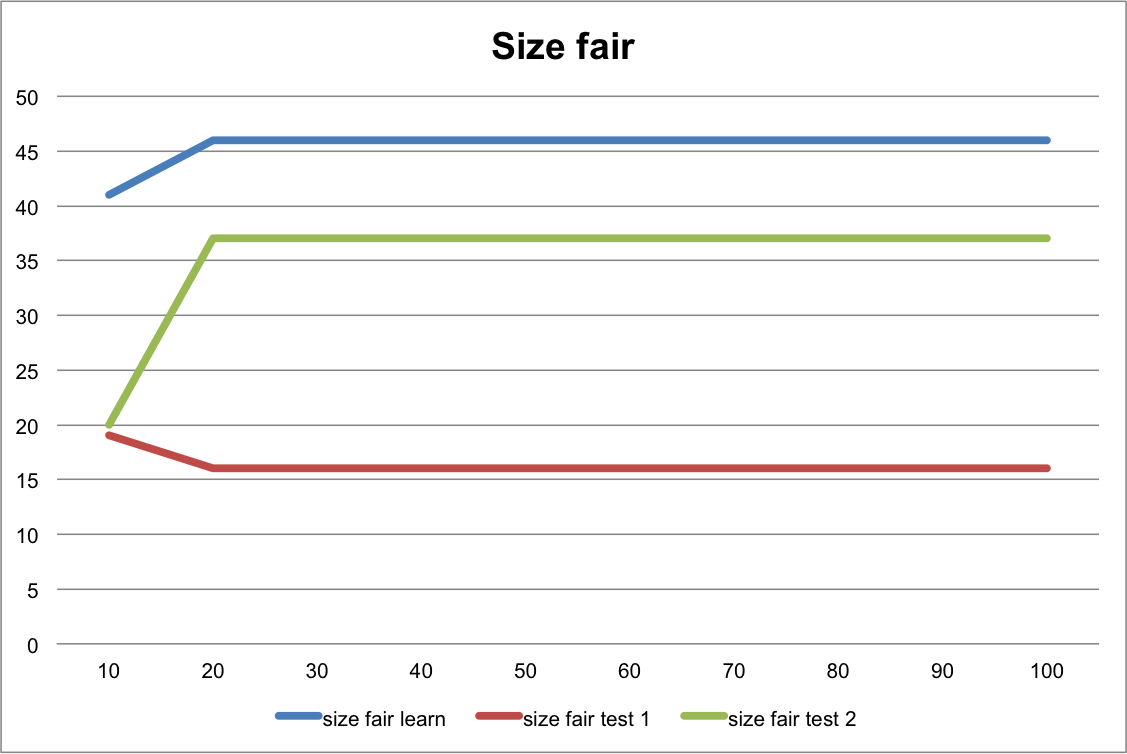
\includegraphics[scale=0.8]{./slike/cross-validation/sizefair.png}
	\caption{Usporedba kvalitete evoluirane jedinke na okolini za učenje i dvije testne okoline za operator križanja koji je pravedan s obzirom na veličinu}
	\label{sizefair}
\end{figure}

\begin{figure}[H]
	\centering
	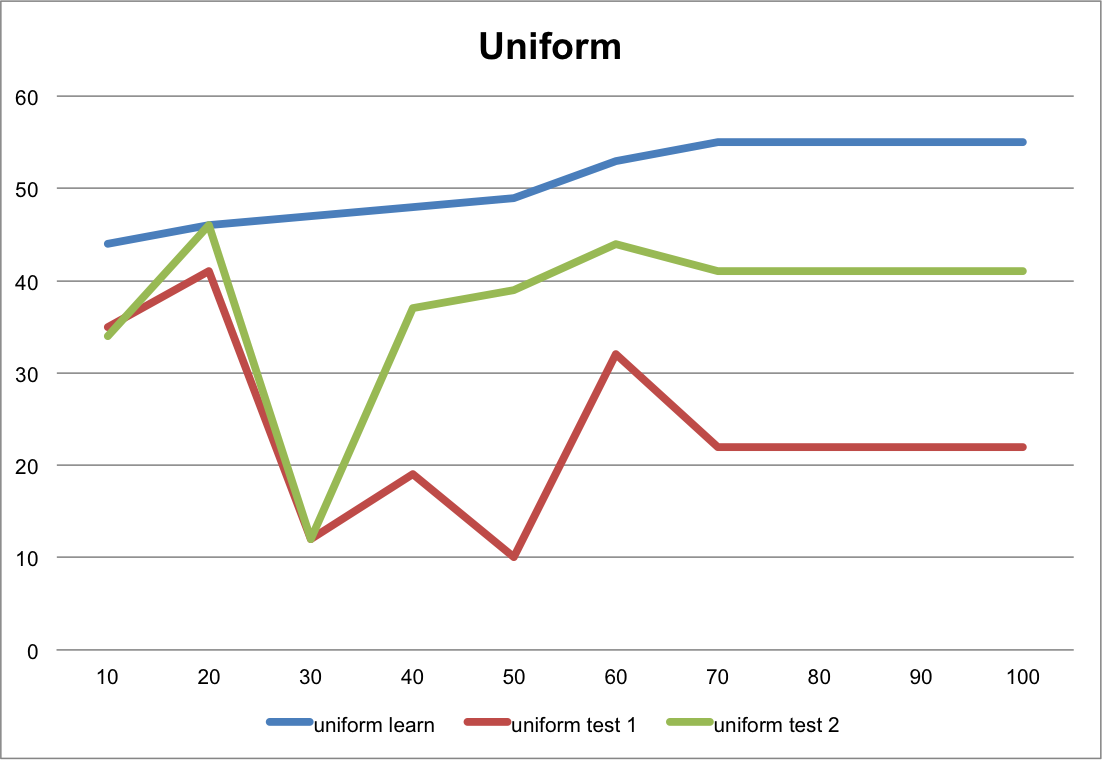
\includegraphics[scale=0.8]{./slike/cross-validation/uniform.png}
	\caption{Usporedba kvalitete evoluirane jedinke na okolini za učenje i dvije testne okoline za uniformni operator križanja}
	\label{uniform}
\end{figure}


\subsubsection{Sveukupni rezultati}
Općenita usporedba svih pojedinačnih operatora križanja prikazana je na tablici \ref{overAllTable}. Tablica za svaki operator prikazuje njegov prosječan rang. Prosječan rang je pritom izračunat kao aritmetička sredina svih rangova koje je taj operator postigao za svaki pojedini problem na kojem je bio testiran.

\begin{table}[H]
 	\centering

    \begin{tabular}{| l | l | l |}
    \hline
   problem & 6 - multiplekser & 11 - multiplekser \\ \hline
   skup završnih znakova & $\{a_0, a_1, d_0, d_1, d_2, d_3 \}$ & $\{a_0, a_1, a_2, d_0, d_1, d_2, d_3, d_4, d_5, d_6, d_7 \}$\\ \hline
   skup nezavršnih znakova & $\{ AND, OR, NOT, IF \}$  & $\{ AND, OR, NOT, IF \}$ \\ \hline
   funkcija dobrote & broj netočnih izlaza & broj netočnih izlaza \\ \hline
    \end{tabular}
    
    \caption{Prosječan rang učinkovitosti operatora križanja za sve zadane probleme}
    \label{overAllTable}
\end{table}


\subsection{Usporedba učinkovitosti kombinacije operatora križanja}

Kako bi se pokazala učinkovitost kombinacija operatora križanja, proveden je eksperiment nad problemom simboličke regresije symb6 (koji se pokazao kao najteži problem koji je rješavan u sklopu ovoga rada). Eksperiment je započeo s uporabom svih operatora križanja od jednom, gdje se svaki pojedini operator koristio s jednakom vjerojatnosti. Nakon toga, oduziman je jedan po jedan operator sve dok se učinkovitost kombinacije mijenjala na bolje. Na grafu \ref{symb6combo} prikazani su rezultati provedenog eksperimenta. Na grafu je izostavljen slučaj u kojem su se upotrijebili svi operatori iz razloga što je prosječna najbolja dobrota u tom slučaju bila znatno veća nego u ostalim slučajevima - kretala se oko broja 250. Prikaz tog rezultata utjecao bi na razlučivost grafa te je iz tog razloga izostavljen. Oznake na grafu imaju sljedeća značenja:

\begin{itemize}
\item{C1 - kombinacija svih operatora izuzev probabilističkog}
\item{C2 - kombinacija svih operatora izuzev probabilističkog i križanja s jednom točkom prekida}
\item{C3 - kombinacija svih operatora izuzev probabilističkog i križanja s očuvanjem konteksta}
\item{C4 - kombinacija svih operatora izuzev probabilističkog, križanja s očuvanjem konteksta i homolognog križanja}
\item{C5 - kombinacija svih operatora izuzev probabilističkog, križanja s očuvanjem konteksta i uniformnog križanja}
\item{C6 - kombinacija svih operatora izuzev probabilističkog, križanja s očuvanjem konteksta i determinističkog križanja}
\item{C7 - kombinacija svih operatora izuzev probabilističkog, križanja s očuvanjem konteksta i križanja pravednog s obzirom na veličinu}

\end{itemize}

\begin{figure}[H]
	\centering
	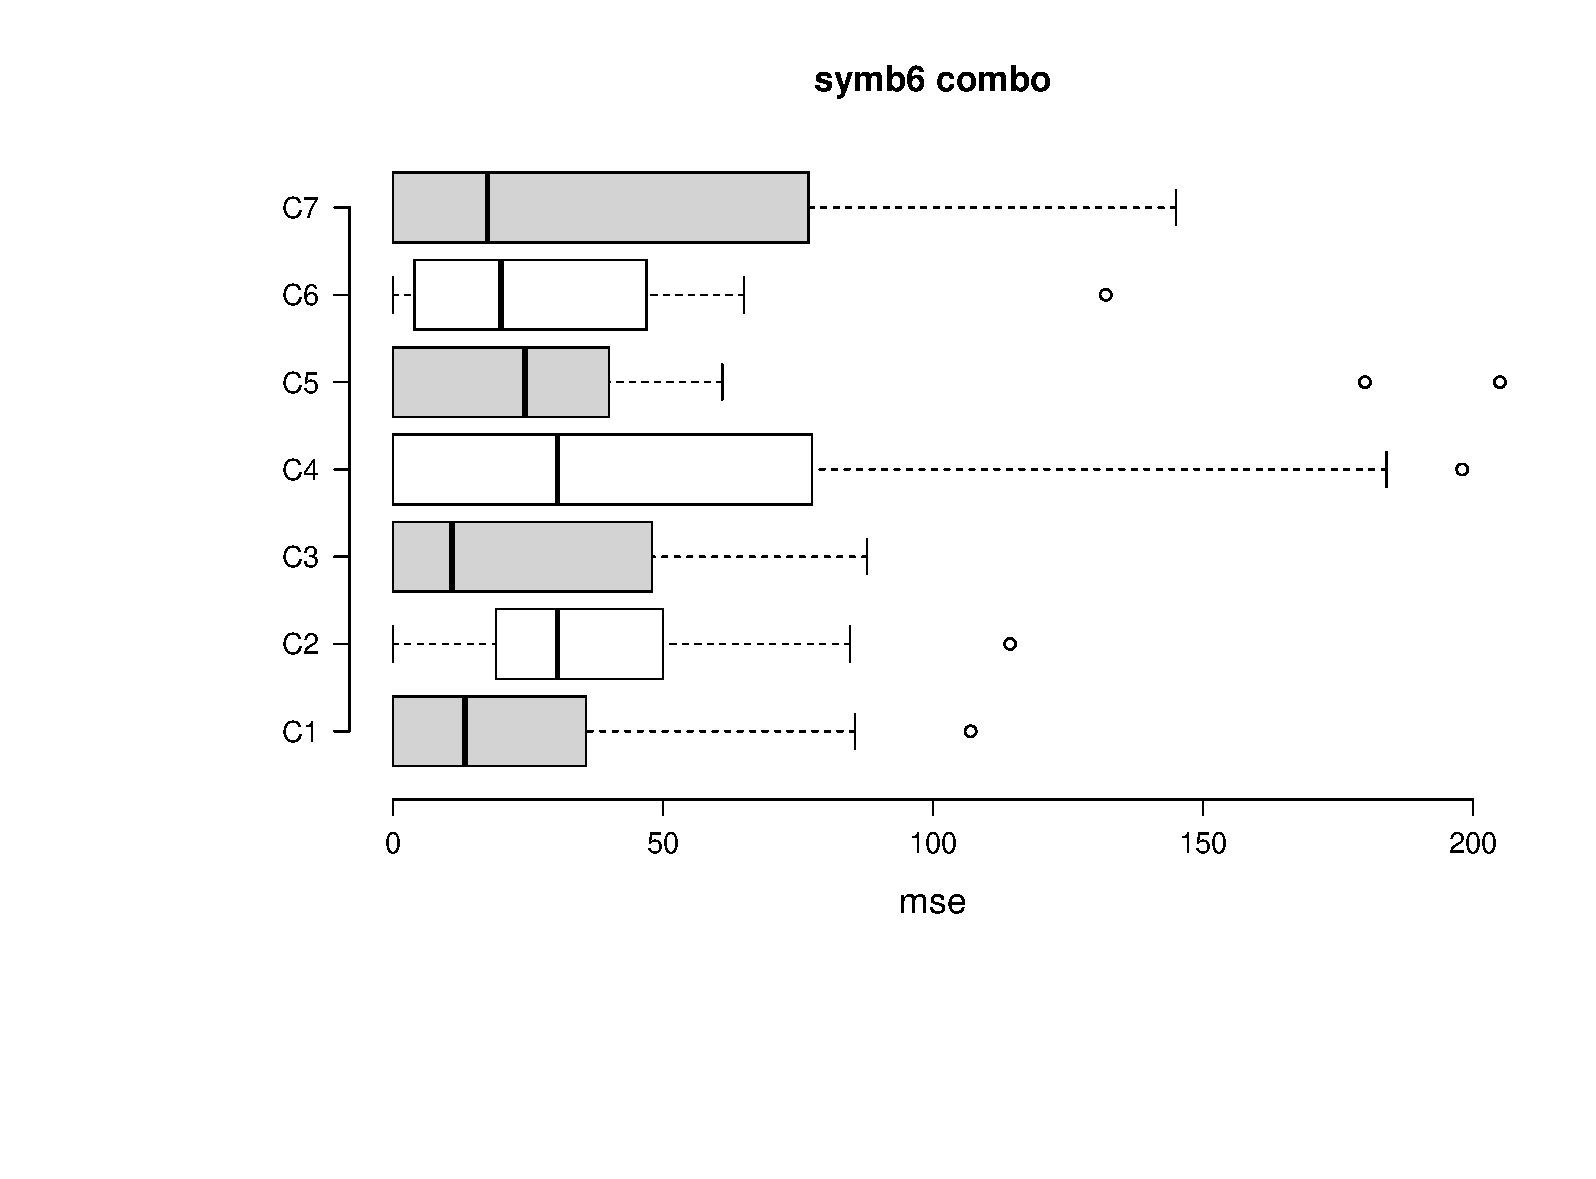
\includegraphics[trim=4cm 4cm 0cm 0cm, scale=0.6]{./slike/boxPlots/symb6-combo.eps}
	\caption{Usporedba učinkovitosti kombinacije operatora križanja na problem simboličke regresije symb6}
	\label{symb6combo}
\end{figure}

Iz dobivenih rezultata vidljivo je, kako je najbolja od svih kombinacija ona koja obuhvaća sve operatore osim probabilističkog i križanja s očuvanjem konteksta. Srednja vrijednost najbolje dobrote ovog operatora iznosi 23.9. Ova vrijednost i dalje je dosta lošija od najbolje dobivene prosječne dobrote s isključivim korištenjem semantičkog i jednostavnog križanja u omjeru 1:9.